% Options for packages loaded elsewhere
\PassOptionsToPackage{unicode}{hyperref}
\PassOptionsToPackage{hyphens}{url}
% !TeX program = pdfLaTeX
\documentclass[12pt]{article}
\usepackage{amsmath}
\usepackage{graphicx,psfrag,epsf}
\usepackage{enumerate}
\usepackage[]{natbib}
\usepackage{textcomp}


%\pdfminorversion=4
% NOTE: To produce blinded version, replace "0" with "1" below.
\newcommand{\blind}{}

% DON'T change margins - should be 1 inch all around.
\addtolength{\oddsidemargin}{-.5in}%
\addtolength{\evensidemargin}{-1in}%
\addtolength{\textwidth}{1in}%
\addtolength{\textheight}{1.7in}%
\addtolength{\topmargin}{-1in}%

%% load any required packages here



% tightlist command for lists without linebreak
\providecommand{\tightlist}{%
  \setlength{\itemsep}{0pt}\setlength{\parskip}{0pt}}



\usepackage[dvipsnames]{xcolor} % colors
\newcommand{\ear}[1]{{\textcolor{blue}{#1}}}
\newcommand{\svp}[1]{{\textcolor{RedOrange}{#1}}}
\newcommand{\rh}[1]{{\textcolor{Green}{#1}}}
\newcommand\pcref[1]{(\cref{#1})}
\usepackage{algorithm,algpseudocode,booktabs}
\usepackage{hyperref}
\usepackage[capitalise]{cleveref}
\usepackage{xr}\externaldocument{logarithmic-lineups-revisions}
\usepackage{subfig}

\IfFileExists{bookmark.sty}{\usepackage{bookmark}}{\usepackage{hyperref}}
\IfFileExists{xurl.sty}{\usepackage{xurl}}{} % add URL line breaks if available
\hypersetup{
  pdftitle={Appendix to Perception and Cognitive Implications of Logarithmic Scales for Exponentially Increasing Data: Perceptual Sensitivity Tested with Statistical Lineups},
  hidelinks,
  pdfcreator={LaTeX via pandoc}}



\begin{document}


\def\spacingset#1{\renewcommand{\baselinestretch}%
{#1}\small\normalsize} \spacingset{1}


%%%%%%%%%%%%%%%%%%%%%%%%%%%%%%%%%%%%%%%%%%%%%%%%%%%%%%%%%%%%%%%%%%%%%%%%%%%%%%

\if0\blind
{
  \title{\bf Appendix to Perception and Cognitive Implications of
Logarithmic Scales for Exponentially Increasing Data: Perceptual
Sensitivity Tested with Statistical Lineups}

  \author{
      }
  \maketitle
} \fi

\if1\blind
{
  \bigskip
  \bigskip
  \bigskip
  \begin{center}
    {\LARGE\bf Appendix to Perception and Cognitive Implications of
Logarithmic Scales for Exponentially Increasing Data: Perceptual
Sensitivity Tested with Statistical Lineups}
  \end{center}
  \medskip
} \fi

\bigskip

\noindent%
 

\vfill

\newpage
\spacingset{1.9} % DON'T change the spacing!

\renewcommand{\thesection}{A}
\setcounter{figure}{0}    
\renewcommand\thefigure{\thesection\arabic{figure}}  
\setcounter{equation}{0}    
\renewcommand\theequation{\thesection\arabic{equation}}

\hypertarget{exponential-growth-rates-and-curvature}{%
\section{Exponential growth rates and
curvature}\label{exponential-growth-rates-and-curvature}}

Let us consider a simple equation which we could use to simulate data
which grows exponentially in \(x\), with optional error term
\(\epsilon\):
\begin{align}y &= \exp\{\beta_1 x + \epsilon\}\quad \text{where}\quad \epsilon \sim N(0, \sigma).\label{eq:simpleexp}\end{align}

\begin{figure}[hb]

{\centering 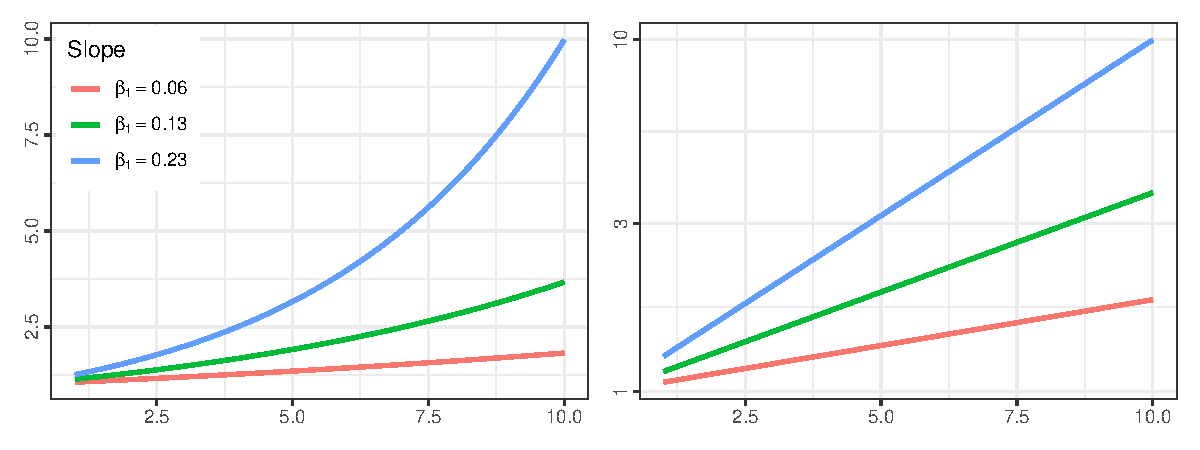
\includegraphics[width=\linewidth,]{appendix_files/figure-latex/simple-exponential-1} 

}

\caption{Linear and log scale simple exponential equations as specified in \cref{eq:simpleexp}, with error term excluded. The y-axis endpoints are a primary visual signal when differentiating between the lines in both plots.}\label{fig:simple-exponential}
\end{figure}

It is important in lineup studies to control for extraneous visual
signals, and when other visual signals creep in, results of the study
can be difficult to interpret \citep{vanderplas_clusters_2017}.

In this particular case, the extraneous visual signals are the endpoints
of the lines (the endpoint at \(x=10\) on a linear scale, and both
endpoints on the log scale), as shown in \cref{fig:simple-exponential}.
Preattentive features guide attention
\citep{wolfeWhatPreattentiveFeature2019}; one of the first things we do
when scanning a graph is to notice the extent of the data within the
axes. We must control the endpoints to ensure that participants are
using active attention to assess the lineup and draw conclusions, so
that the whole visual signal is processed as part of the lineup
evaluation; if participants are making decisions off of the endpoints,
then we cannot interpret the results to say that they are assessing the
rate of exponential growth rather than the end result.

There are several different options for controlling the visual signal in
a lineup:

\begin{enumerate}
\def\labelenumi{\arabic{enumi}.}
\setcounter{enumi}{-1}
\tightlist
\item
  Do nothing and set each subplot's limits to the overall maximum
  limits.
\item
  allow each subplot to have different axis limits
\item
  truncate the displayed range of each subplot to the minimum range
  generated in the lineup
\item
  add extra parameters to the exponential equation to adjust the range
  of the data so that it fits within a pre-specified domain, as in
  \cref{alg:lineup-exponential-data-simulation-algorithm}.
\end{enumerate}

\begin{figure}[tbp]

{\centering 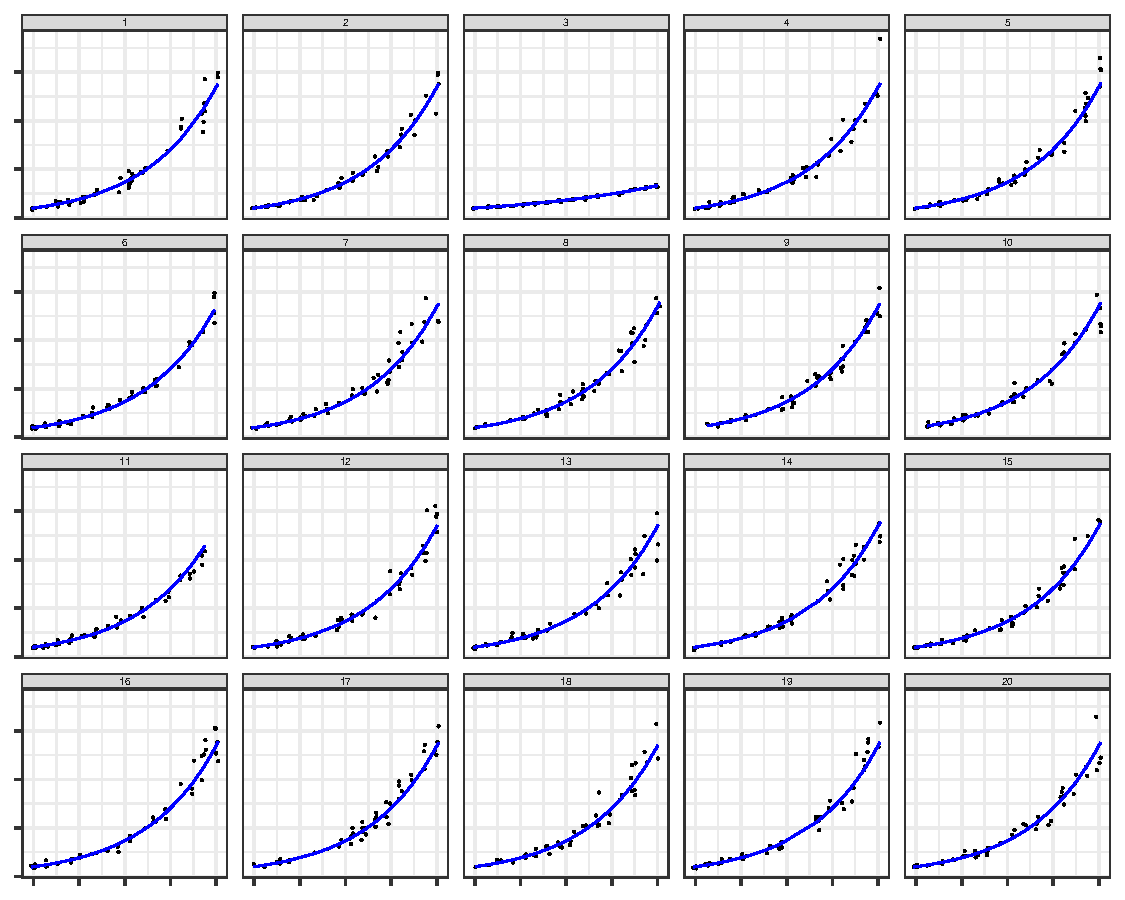
\includegraphics[width=.6\linewidth,]{appendix_files/figure-latex/lineup-fixed-scales-1} 

}

\caption{When axis limits are fixed to the most expansive extent in the generated data, the primary signal becomes the extent of the domain which has data, rather than the growth rate itself.}\label{fig:lineup-fixed-scales}
\end{figure}

Typically, lineups do not show axis labels or scaling, because the goal
is to assess the signal from the data without additional context. In
addition, the traditional 20-panel lineup would be quite visually
confusing in this circumstance:

\begin{figure}[tbp]

{\centering \subfloat[Lineup\label{fig:lineup-free-scales-1}]{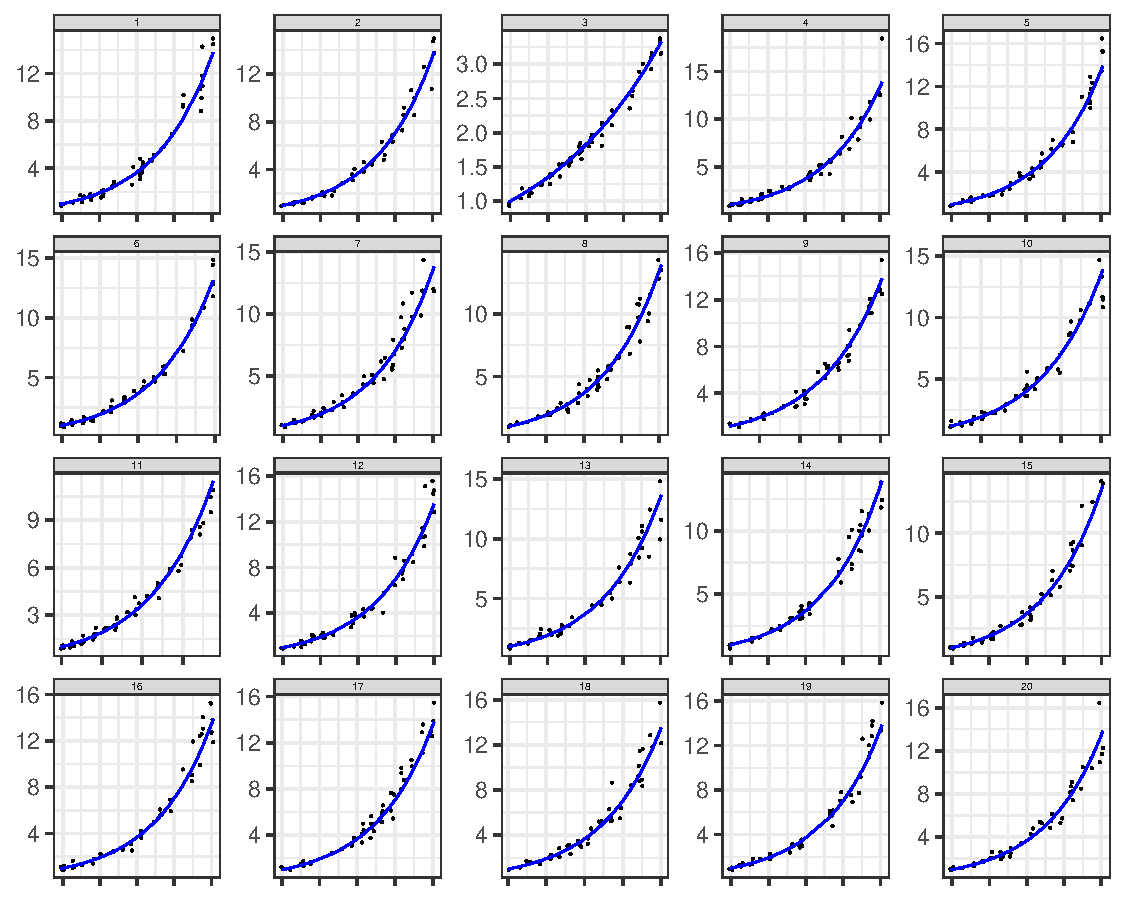
\includegraphics[width=.6\linewidth,]{appendix_files/figure-latex/lineup-free-scales-1} }\subfloat[Overlay of null and signal panels.\label{fig:lineup-free-scales-2}]{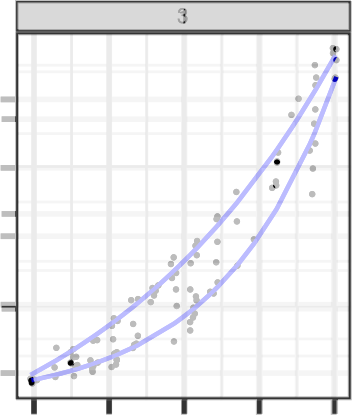
\includegraphics[width=.2\linewidth,]{images/curvature-overlay-free-scales} }

}

\caption{When y-axis limits vary by panel, the y-axis labels are the primary visual signal; the secondary signal (when the panels are overlaid) is the curvature of the line.}\label{fig:lineup-free-scales}
\end{figure}

\cref{fig:lineup-free-scales} demonstrates that when we ignore the
y-axis labels and overlay the signal panel with one of the null panels,
the remaining difference is the curvature of the line. If we want to
keep the standard convention of not including y-axis labels in lineups
for simplicity and to reduce plot clutter, this alternative signal seems
promising (and as we will show, is approximately equivalent to option
3).

Let us next consider option 2: Crop each panel to the minimum limits of
all generated data. The result is shown in
\cref{fig:lineup-truncate-scales}. This operation shifts which axis
becomes the visually important factor, but doesn't change the problem:
previously the issue was the y-axis extent, now it is the x-axis extent.
Both of these parameters are implicitly affected by how we generate
exponential data. In order to truly assess whether people can
discriminate between comparable exponential growth rates graphically, it
is more useful to approach the problem from a curvature perspective
rather than to artificially limit the data shown.

This issue is a fundamental problem when testing graphics: the test must
meet the ``goldilocks'' standard - not too hard, not too easy, but just
right. Both option 0 and option 2 fail this standard.

\begin{figure}[tbp]

{\centering 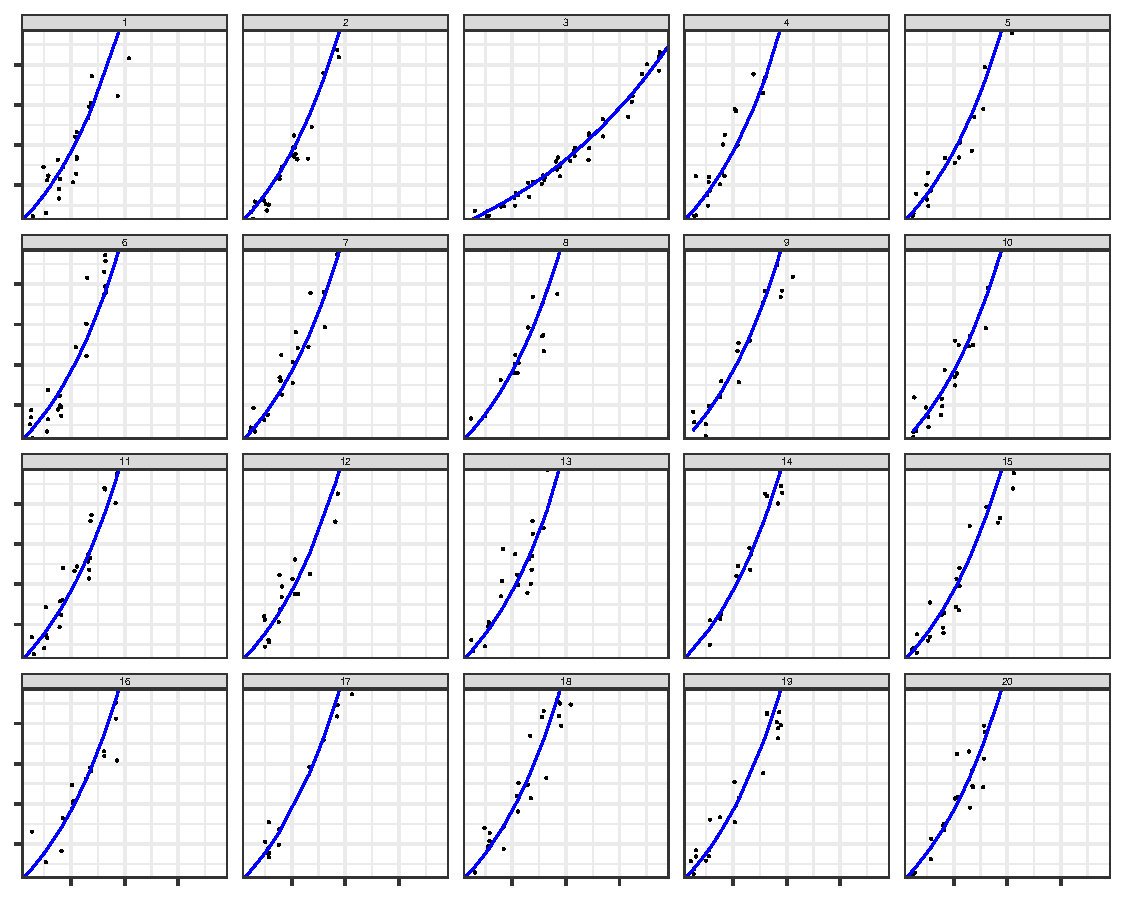
\includegraphics[width=.6\linewidth,]{appendix_files/figure-latex/lineup-truncate-scales-1} 

}

\caption{When axis limits are fixed to the most restrictive in all generated data, the primary signal becomes the extent of the x axis which is covered with data, rather than the growth rate itself.}\label{fig:lineup-truncate-scales}
\end{figure}

Visually, both the \(x\) and \(y\) axes matter equally, even if it might
on paper make sense to truncate \(x\) in order to control the \(y\) axis
range.

An additional benefit of controlling endpoints is that it also provides
some realism: our goal was to assess the ability to examine exponential
growth \textbf{rates}, motivated by the COVID-19 pandemic. As each
geographic reporting region started with different numbers of cases and
had different control policies, the \(\alpha\) and \(\theta\) parameters
are reasonable to represent some of these differences while still
examining the underlying exponential behavior.

To control these endpoints on both scales then we have to move to an
exponential model that is a bit more complicated:
\begin{align}y = \alpha \cdot \exp\left\{\beta_1 x + \epsilon\right\} + \theta\quad \text{where}\quad \epsilon \sim N(0, \sigma).\label{eq:complexexp}\end{align}

\(\alpha\) and \(\theta\) were used to make endpoints consistent among
the growth rates. As a result, the lineups examine the degree of
inflection of the trend rather than the explicit exponential growth
rate. An explanation for how the ultimate values for \(\alpha\) and
\(\theta\) were determined is provided in
\cref{alg:lineup-exponential-data-simulation-algorithm}.
\cref{fig:lineup-scale-data} uses the parameters in
\cref{tab:parameter-data} and the data generating method described in
\cref{alg:lineup-exponential-data-simulation-algorithm}. The result is a
series of panels which have obvious variation due to the points (a
desirable feature) but where the underlying relationship shown in blue
has consistent endpoints. As a result, the question becomes whether
participants can identify that plot 3 has a different growth rate (as
measured by the curvature of the line).

\begin{figure}[tbp]

{\centering 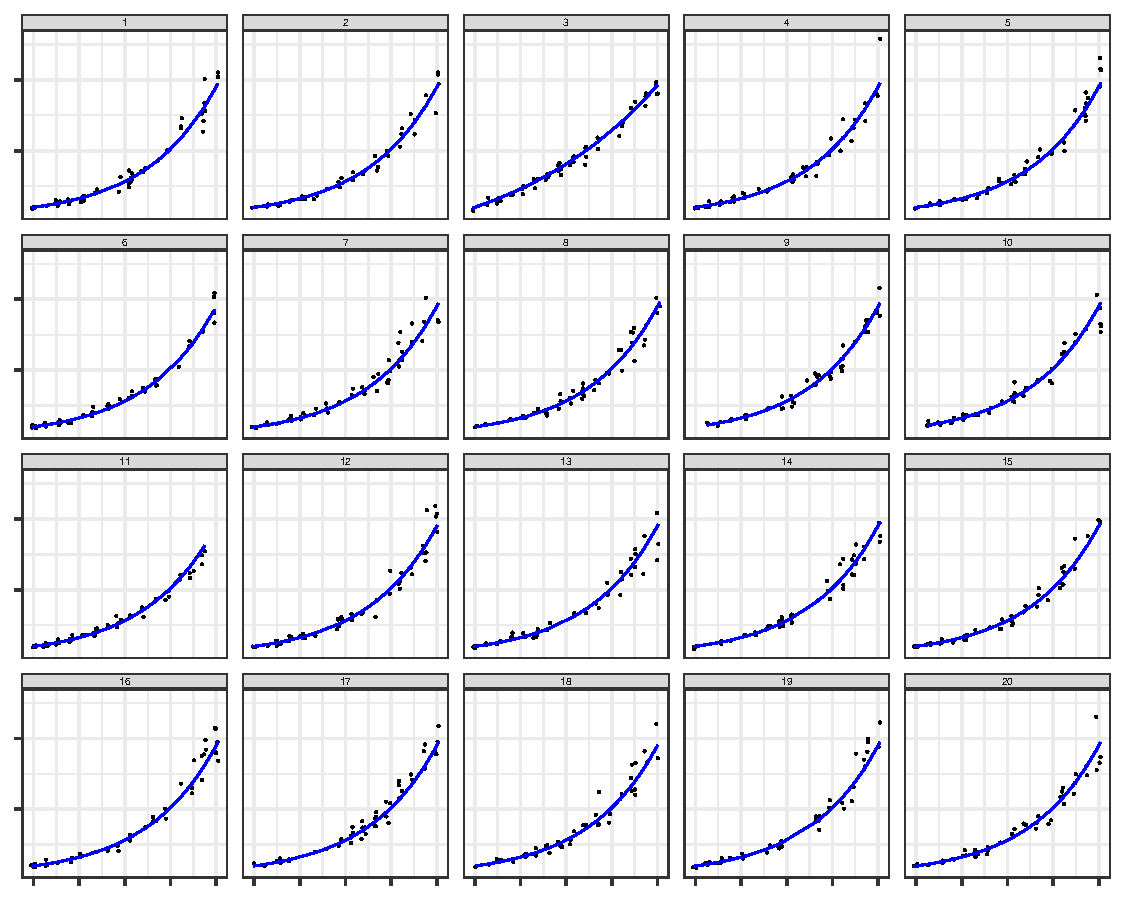
\includegraphics[width=.6\linewidth,]{appendix_files/figure-latex/lineup-scale-data-1} 

}

\caption{When the data are scaled such that endpoints are similar across all conditions, the primary feature becomes the curvature of the line, while individual plots show random variation due to the scatter around the line.}\label{fig:lineup-scale-data}
\end{figure}

\renewcommand{\thesection}{B}

\hypertarget{rorschach-lineup-evaluation}{%
\section{Rorschach Lineup
Evaluation}\label{rorschach-lineup-evaluation}}

In addition to the experimental lineups, we generated three sets of
homogeneous ``Rorschach'' lineups, each featuring panels simulated from
the same distribution. Importantly, participants were unaware that there
was no designated target panel for identification.
\cref{fig:rorschach-lineups} illustrates the selection proportions for
each panel on the ``Rorschach'' lineups corresponding to different
curvature combinations and replicated datasets, when presented on both
log and linear scales. Notably, the panel number is irrelevant, and the
darker shade (bottom) denotes panels chosen more frequently than others.

This approach allows us to explore whether any null panels were
significantly more unique, providing insights into the null plot
sampling method. The plots exhibit a relatively even distribution,
offering multiple candidates for the most interesting panel. It is worth
noting that in the low curvature ``Rorschach'' lineups simulated in data
set replication one, a single panel stands out, with over 50\% of
participants selecting the same null panel on the linear scale and just
under 50\% on the log scale. Through a visual examination of
``Rorschach'' evaluations, we determined that our null sampling method
is appropriate.

\begin{figure}[tbp]

{\centering 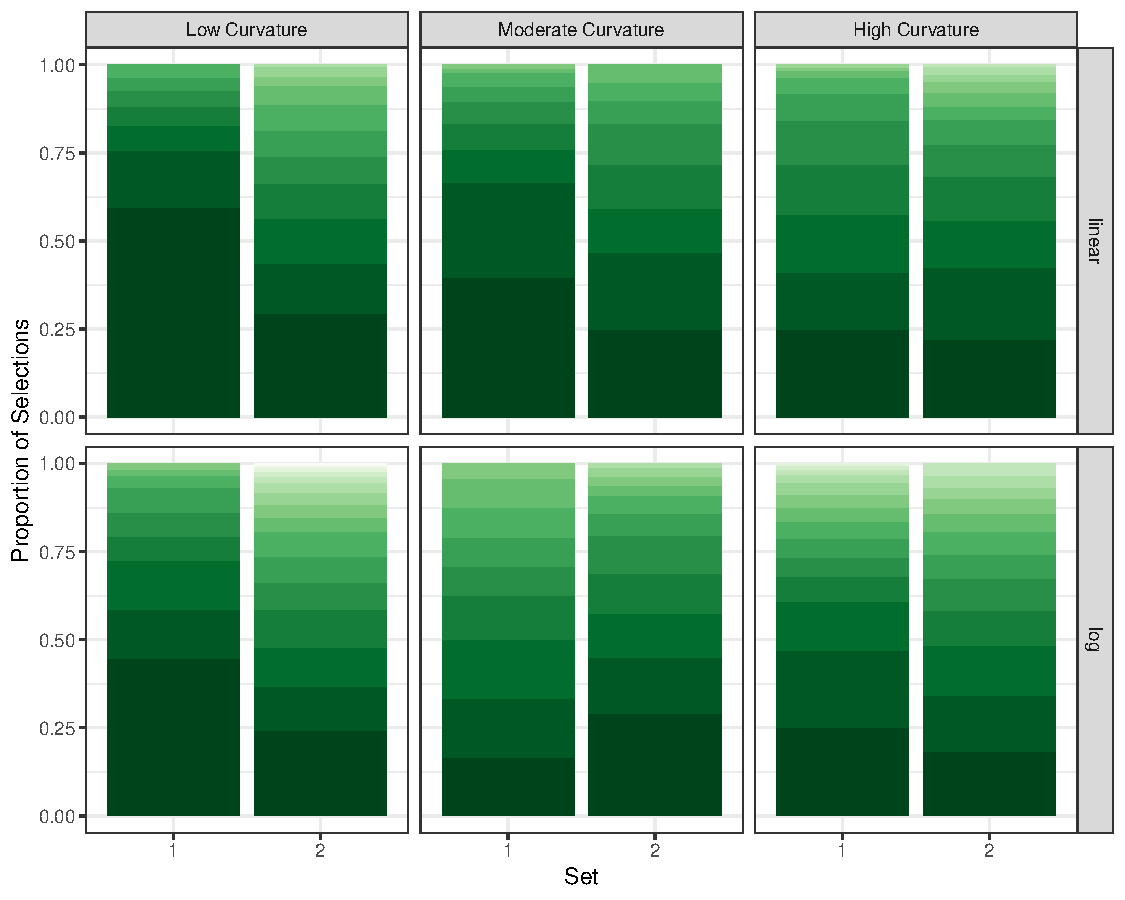
\includegraphics[width=.6\linewidth,]{appendix_files/figure-latex/rorschach-lineups-1} 

}

\caption{When axis limits are fixed to the most restrictive in all generated data, the primary signal becomes the extent of the x axis which is covered with data, rather than the growth rate itself.}\label{fig:rorschach-lineups}
\end{figure}

\renewcommand{\thesection}{C}

\hypertarget{participant-self-percieved-confidence-and-accuracy}{%
\section{Participant self-percieved confidence and
accuracy}\label{participant-self-percieved-confidence-and-accuracy}}

In addition to investigating how scale and curvature rate influence
participant accuracy, we asked participants to indicate their level of
confidence on a five-point likert scale by answering, ``How certain are
you?'' \cref{fig:conf-mosaic} shows the observed confidence rating
proportions for correct and incorrect identifications across the
different scale and curvature combination scenarios. Overall,
participants who correctly identified the target plot were more
confident in their plot choice across all conditions with the highest
confidence levels and accuracy in scenarios with large differences in
curvature between the target and null panels.

\begin{center}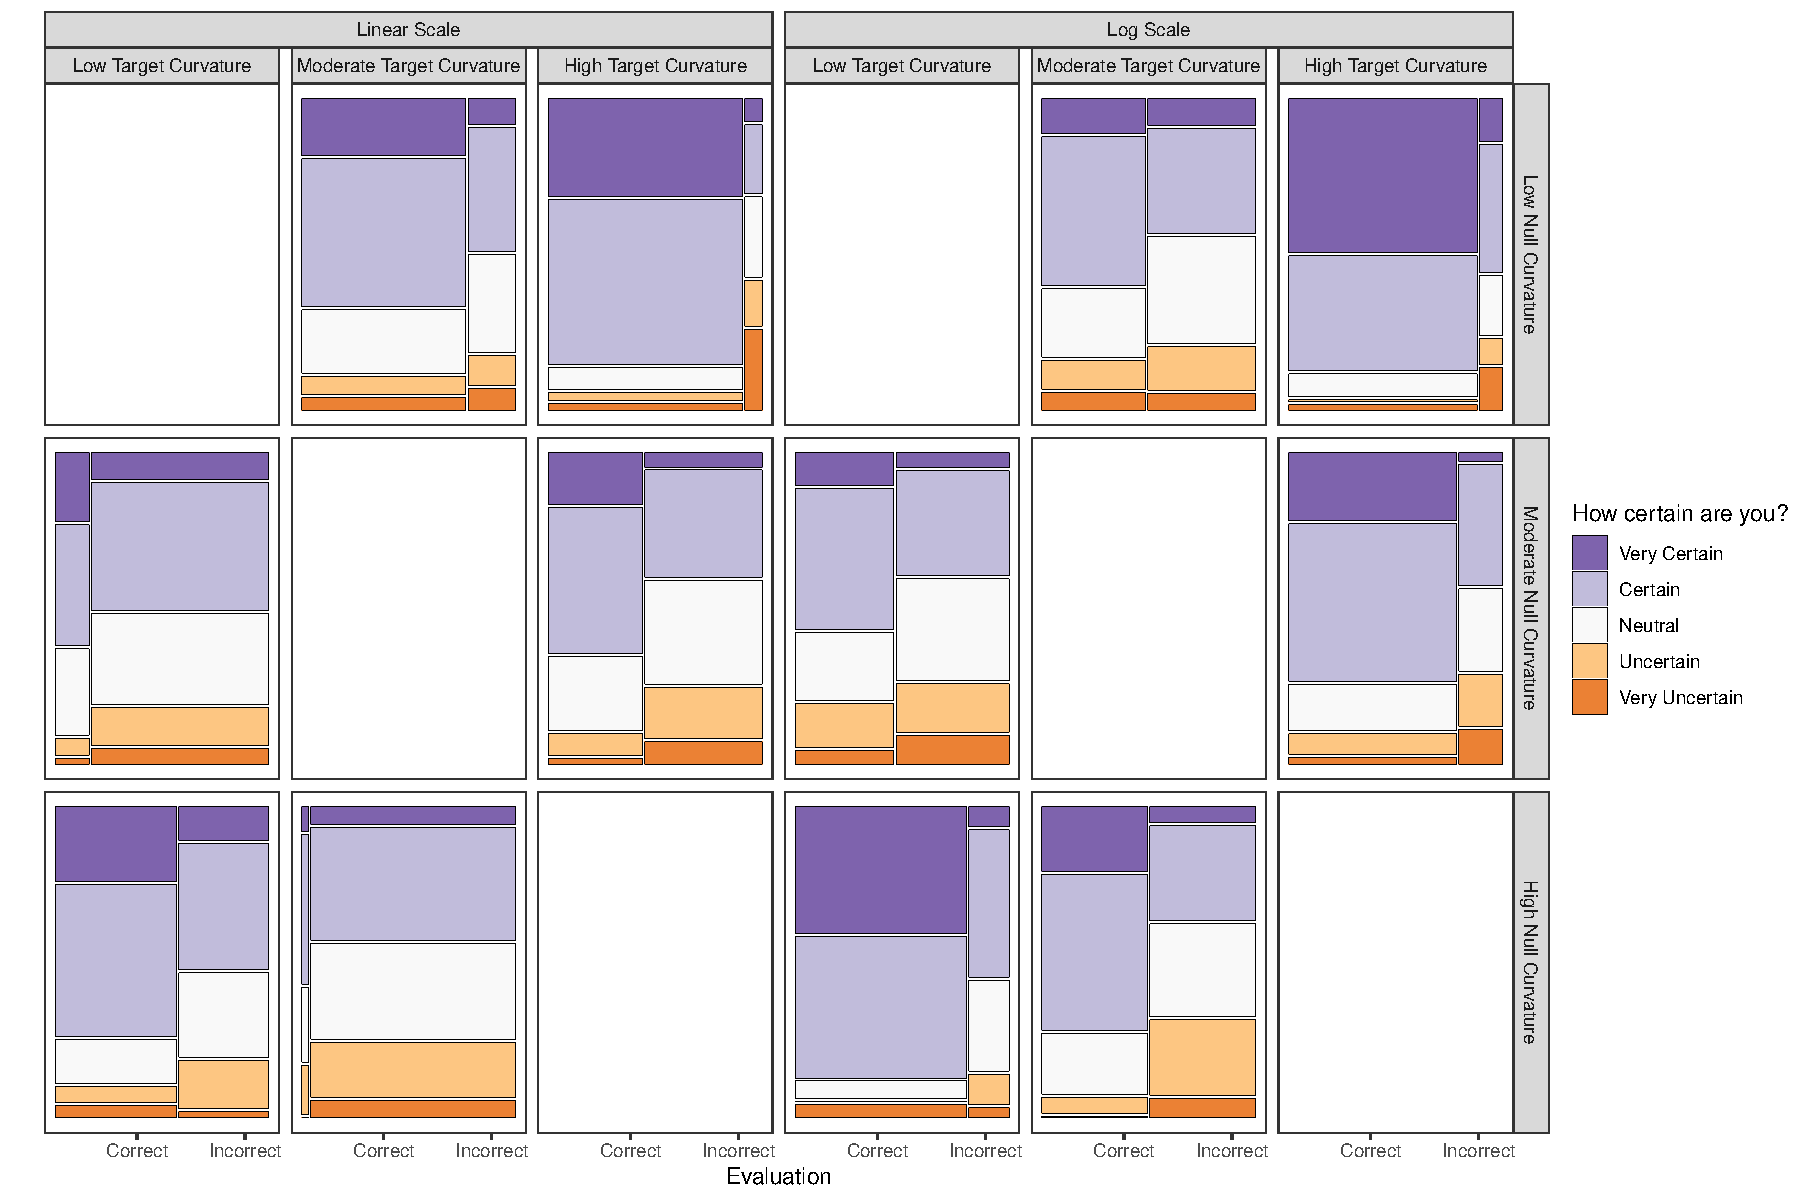
\includegraphics[width=\linewidth,]{appendix_files/figure-latex/conf-mosaic-1} \end{center}

\bibliographystyle{plain}
\bibliography{bibliography.bib}



\end{document}
